\chapter{Testování}

Každý správný vývojový cyklus software obsahuje fázi testování\cite{zivotnicyklus}. Aplikaci lze testovat ve~více vlnách, kdy se pokaždé provádí jiný typ testů. Obecně lze testy rozdělit do dvou hlavních skupin - blackbox a whitebox.

Blackbox testy testují aplikaci zvenku a nepotřebují vědět, co se děje uvnitř. Proto se testy označují jako \uv{blackbox}. U těchto testů je aplikace černou skříňkou a jsou k dispozici pouze dva otvory - vstup a výstup. Do aplikace se pošle nějaký vstup a očekává se určitý výstup. Pokud výstup splňuje očekávání, test byl úspěšný. Hlavní výhodou těchto testů je jejich jednoduchost, protože není potřeba znát konkrétní obsah tříd a metod uvnitř aplikace. Do blackbox testů lze zařadit testy rozhraní (Selenium \cite{selenium}), akceptační nebo zátěžové.

Naproti tomu whitebox testy vyžadují znalost kódu aplikace a jsou pevněji svázány s~implementací uvnitř. Tyto testy jsou mnohem konkrétnější a obvykle testují menší celky aplikace (balíčky -$>$ třídy -$>$ metody). Postup testování může být dvojí. Buď se testují nejdřív největší celky a postupně se zanořuje, nebo se naopak postupuje od nejmenších jednotek po ty největší. Těmto testům se říká jednotkové (angl. unit testy). Do kategorie whitebox testů spadají také integrační testy, které ověřují, zda spolu jednotlivé komponenty aplikace komunikují tak, jak mají.

\section{Použitý způsob testování}

Testování této aplikace není tak snadné jako u webových aplikací. Některé testy nejsou realizovatelné (např. testy rozhraní pomocí nástroje Selenium), protože aplikace není spustitelná v prohlížeči. Toto omezení způsobuje globální objekt Titanium, který není v prostředí prohlížeče k dispozici a aplikace se tak stává nepoužitelnou.

Pro testování je využita JavaScriptová knihovna jsUnity\cite{jsunity}, pomocí které jdou poměrně snadno vytvářet jednotkové testy. Poskytuje jednak běhové prostředí a hlavně assertovací metody, které ověří výsledek testu. Knihovnu je potřeba trochu poupravit, aby výsledek testů vypsala do okna a ne do standardního výstupu, kde by se výsledek ztratil v záplavě runtime hlášení.

Testy jsou seskupeny v objektech, které se spouští metodou \emph{jsUnity.run()}. Aby nebyly při každém testu znovu zakládány všechny objekty, vytvoří se předem, a během testů už se na nich pouze volají metody. Korektní postup je sice jejich zakládání před každým testem v metodě \emph{setUp()}, ale tento způsob se ukázal jako hodně pomalý a bylo od něj upuštěno. Nejpomalejší operace je určitě založení spojení s databází, která je potřeba u většiny testů, a protože testy mají být hlavně rychlé, bylo nutné zvolit nějaký kompromis.

\section{Testování asynchronních volání}

V aplikaci se mnoho operací děje asynchronně, aby aplikace nezamrzala (hlavně při spojení se vzdálenými servery). Tento způsob běhu aplikace bohužel znemožňuje testování jednotkovými testy. Jak vypadá asynchronní volání ukazuje diagram \ref{fig:async-tests}.

\begin{figure}[h]
\begin{center}
	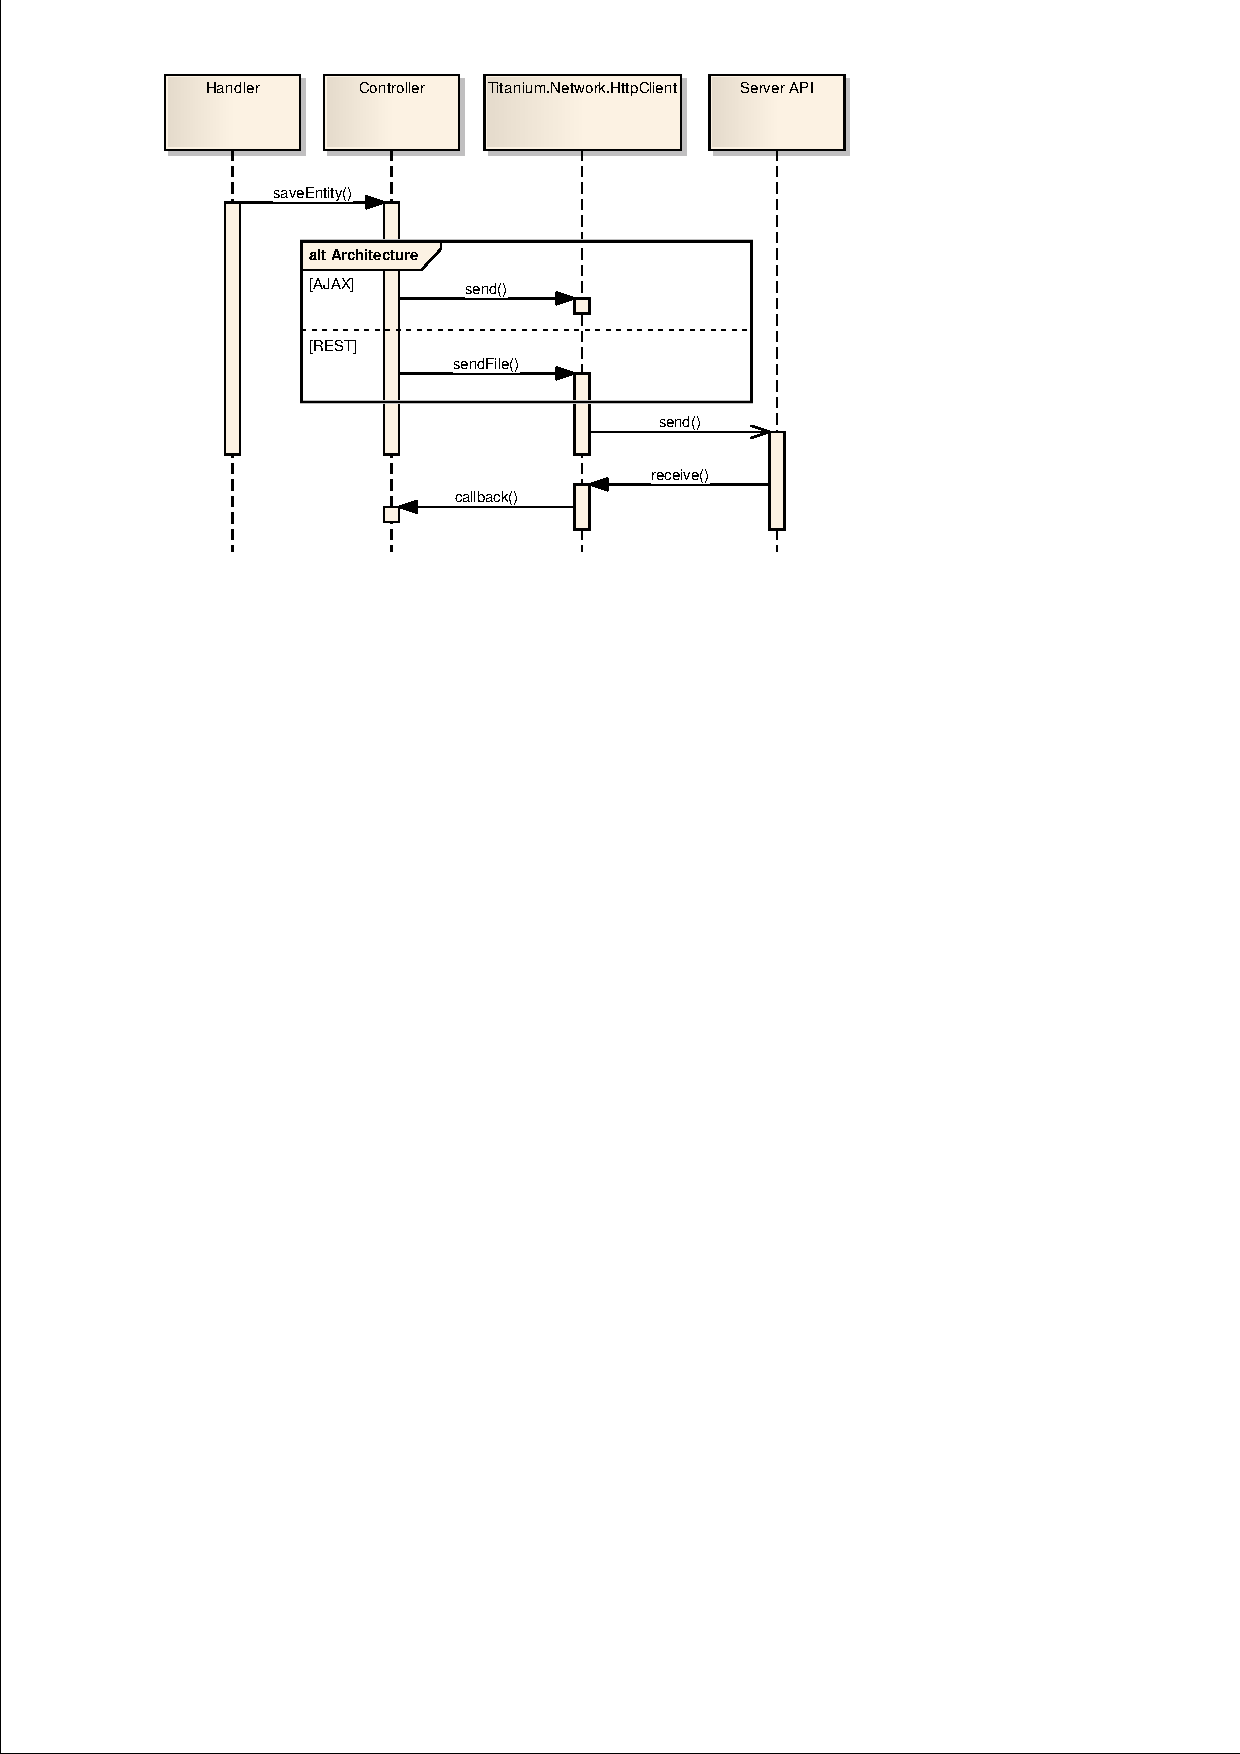
\includegraphics[width=15cm,trim=10mm 205mm 40mm 10mm, clip]{figures/async-tests}
	\caption{Asynchronní volání}
	\label{fig:async-tests}
\end{center}
\end{figure}

Problém, který zabraňuje testování, vzniká v kroku č.3 - předání callbacku. Během testování se o volání metod stará běhové prostředí a není možné volat jednotlivé metody (testy) samostatně. Důsledkem tohoto chování je nemožnost \uv{vrátit} se z HTTP klienta zpět do testu a vyhodnotit správnost odpovědi.

\section{Zátěžové testy}

Součástí fáze testování této práce jsou také zátěžové testy, jejichž úkolem je ověřit, jak rychle některé operace probíhají. Jako operace byla zvolena ta, která je využívána nejčastěji, a sice výpis úkolů z daného projektu. Při používání aplikace se totiž ukázalo, že tato akce trvá poměrně dlouho, a zátěžové testy by mohly ukázat, jak moc závažný problém to je.

Zátěžové testy jsou postaveny na podobném principu jako jednotkové testy, až na to, že zde se nesleduje výsledek testu, ale pouze jeho průběh. Test probíhá ve více iteracích, aby byla zátěž vystupňována. Bylo vytvořeno celkem 7 scénářů, které byly postupně otestovány:

\begin{itemize}
\item prázdný úkol (bez štítků a přiřazení)
\item úkol s jedním štítkem
\item úkol se dvěma štítky
\item úkol přiřazený uživateli s jedním štítkem
\item úkol přiřazený uživateli se dvěma štítky
\item úkol přiřazený uživateli s pěti štítky
\item úkol přiřazený uživateli s deseti štítky
\end{itemize}

Součástí každé iterace je vložení dalšího úkolu (příp. se štítky a uživatelem) do databáze a zavolání metody, starající se o načítání úkolů z databáze. Tím postupně narůstá zátěž, protože počet úkolů v databázi roste. Iterací bylo při každém testu celkem padesát. Čas spotřebovaný v rámci jedné iterace je měřen pomocí objektu \emph{Date} a jeho metody \emph{getTime()}. Tento čas je posléze vypsán na výstup a je dále ručně zpracováván. Hrubá data z těchto testů jsou uvedena v přílohách této práce. Z těchto změřených dat byl také pro lepší názornost vytvořen graf, který je vložen níže. Jeho průběh není zcela hladký, což způsobuje pravděpodobně fakt, že testovací prostředí není úplně izolované od dalších procesů běžících na stejném počítači a procesor tak může dát prioritu jiné aplikaci a test se zpomalí. Dalším důvodem může být to, že je nutné číst data z pevného disku (databáze), což může ve stejnou chvíli chtít víc aplikací. Aplikace se tedy chová dle očekávání, protože graf zátěže stoupá lineárně. V grafu nelze pozorovat ani žádné extrémní výkyvy, které by ukazovaly na nějaké závažnější problémy.

\begin{figure}[h]
\begin{center}
	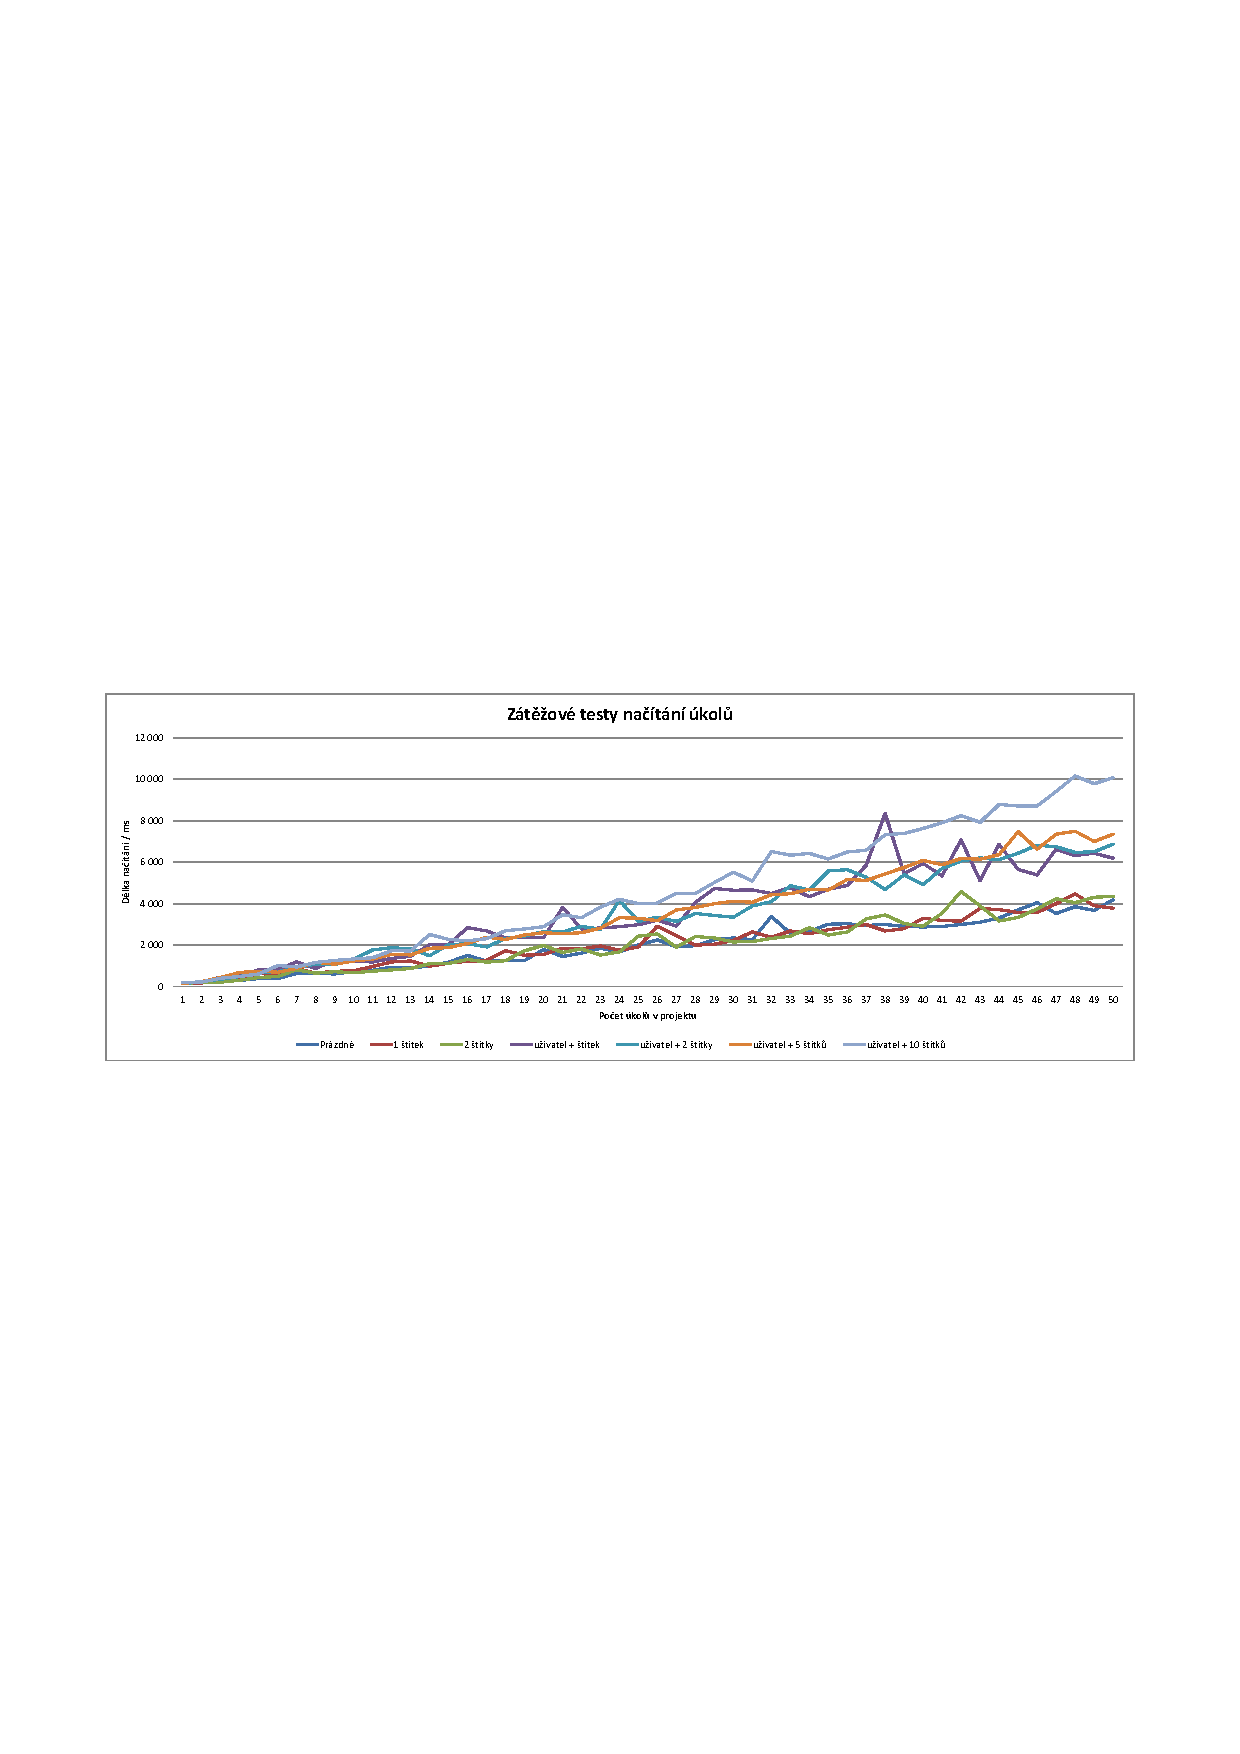
\includegraphics[trim=15mm 115mm 15mm 110mm, clip, width=15cm]{figures/zatezove-testy}
	\caption{Zátěžové testy}
	\label{fig:load-tests}
\end{center}
\end{figure}

\section{Akceptační testy}

V rámci fáze testování byly provedeny také akceptační testy, jejichž cílem bylo objektivně posoudit splnění požadavků. Tyto testy nevyžadují žádné zvláštní nástroje a běhová prostředí, stačí tužka a papír. Hlavním podkladem pro ně jsou vypracované user stories, které byly rozepsány v kapitole 3 - Analýza. Výsledky testů jsou v tabulce \ref{tab:failed-accept-tests}, kde jsou vypsány kvůli lepší přehlednosti pouze nesplněné user stories. Všechny ostatní lze tedy považovat za splněné.

\begin{table}[h]
\begin{center}
	\begin{tabular}{| c | p{5cm} | p{5cm} |}
	\hline
	Role & User story & Důvod nesplnění \\
	\hline
	\hline
	Uživatel \slash vývojář & Spárovat úkol s konkrétním commitem do repozitáře & Přehled commitů lze získat pouze z GitHubu, ostatní servery toto neumožňují \\
	\hline
	Uživatel \slash vývojář & Exportovat úkol a poslat ho jednoduše kolegovi v týmu, aby ho nemusel ručně přepisovat & Funkce se ukázala jako redundantní. O notifikaci se postará verzovací server. \\
	\hline
	Uživatel \slash  vývojář \slash  senior & Být informován o změnách v mých repozitářích na serverech & Tuto funkci opět umožňuje pouze GitHub \\
	\hline
	Uživatel \slash  vývojář \slash  junior & Být informován o nově přiřazených úkolech od senior vývojářů & Není nutné, postará se verzovací server \\
	\hline
	\end{tabular}
\end{center}
\caption{Přehled nesplněných user stories}
\label{tab:failed-accept-tests}
\end{table}